\section{Existerande Raviolimaskiner}
De Raviolimaskiner som finns på marknad innehåller två huvuddelar, en pump för fyllning och en motordriven degform. 

Ett exempel på en Raviolimaskin visas på Figuren~\ref{raviolihemma}. Den består av två cylindriska degformar och en lucka där man fyller maskinen med fyllningsmaterial. Maskinens degfomar fungerar även som pump genom att de drar in fyllningsmaterialet när man snurrar dem m.h.a. ett handtag eller en motor.
 	\begin{figure}[h]
 		\begin{center}
 			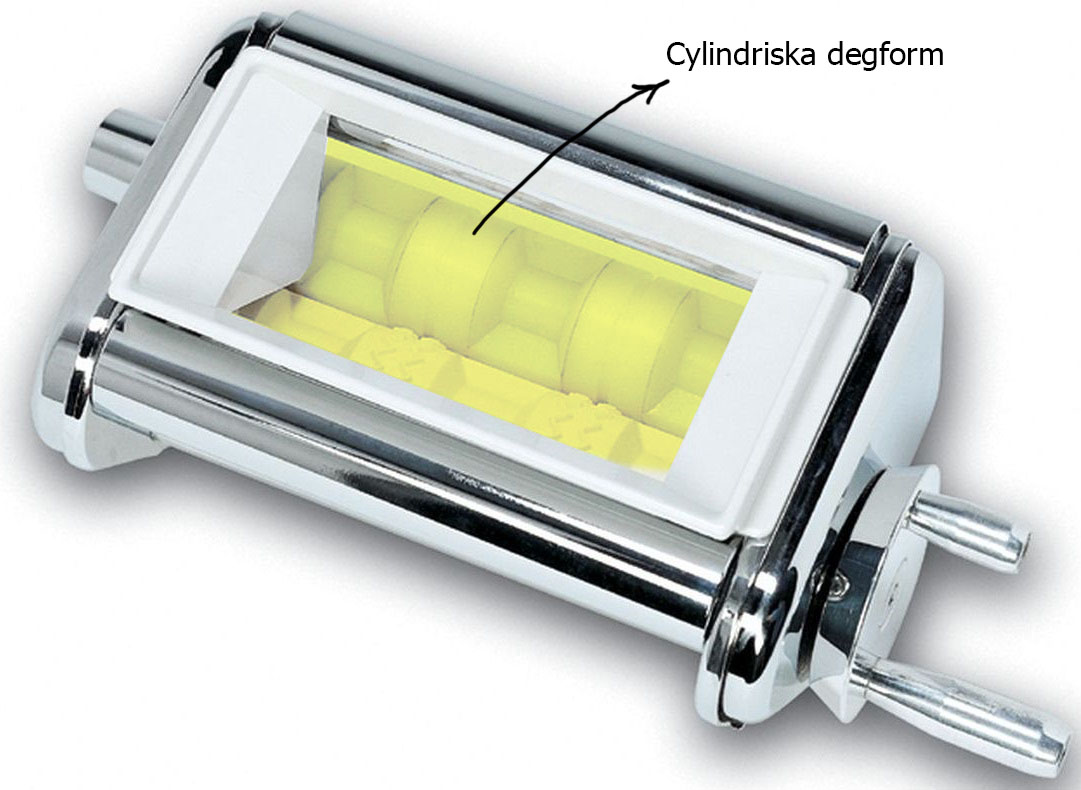
\includegraphics[scale=0.4]{images/ravioli_machine_comment.jpg}
 			\caption{Raviolimaskin bestående av två cylindriska degformar~\cite{raviolimaskinbutik} }
 			\label{raviolihemma}	
 		\end{center}
 	\end{figure}
 
Den industeriella Raviolimaskinen som figur~\ref{pastamaskin} visar, fungerar med samma princip som maskinen på figur~\ref{raviolihemma}. Denna maskin gör allt från placering av en Raviolideg på maskinens degform till den slutar degen automatiskt.

Ett annat exempel på en industriell Raviolimaskin visas på figur ~\ref{industraviol_2}. Denna maskin består av en pump, en degform och en rullbana. Den typen av maskin fyller en Ravioli i tag och placering av Raviolideg på maskinen degform görs manuellt.
   .
 \begin{figure}[ht]
 	\begin{center}
 		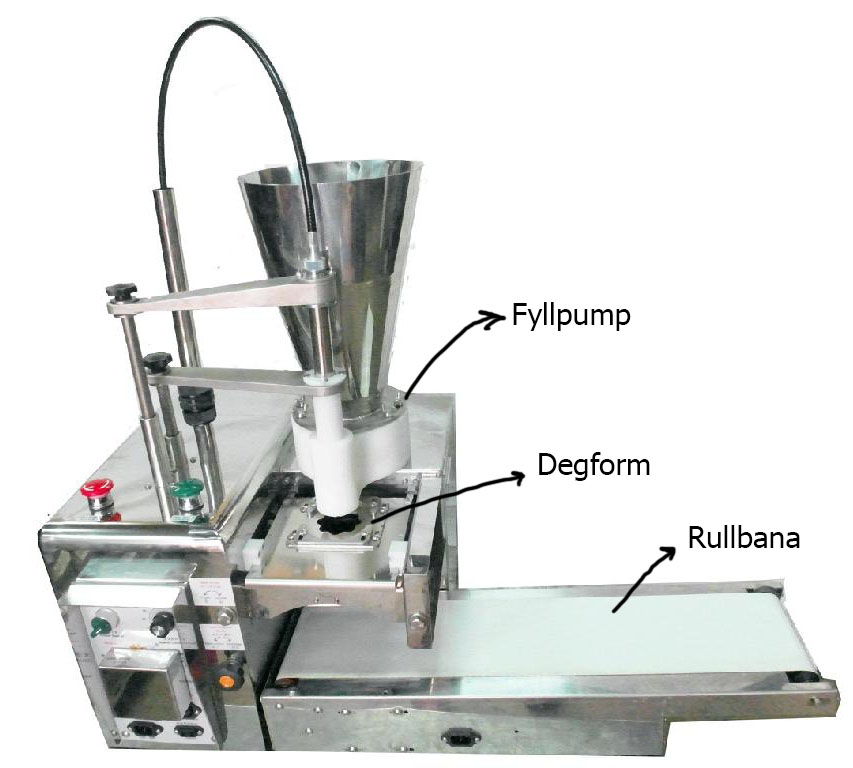
\includegraphics[scale=0.4]{images/industriell_machine_comment.jpg}
 		\caption{Industriell Raviolimaskin som gör en Ravioli i tag(ref)}
 		\label{industraviol_2}	
 	\end{center}
 \end{figure}
 
 

 